%-------------------------------------------------------------------------------
\section{Evaluation}
\label{s:eval}
%-------------------------------------------------------------------------------

We explore the performance of \schedbe{} in relation to the following questions:
\begin{enumerate}
    \item Does the new \schedbe{} isolate LC from BE workloads?
    \item Is parking necessary?
    \item How much does the patch cost?
\end{enumerate}

All the graphs in this paper run on Linux version 6.14.2, the baseline version
that our patch builds on. \hmng{TODO put in specs of ..? zg machines? I didn't
always use all of the cores, but ig I can say that on a per-experiment basis}

\subsection{Does \schedbe{} isolate?}

\begin{figure}[t]
    \centering
    \begin{subfigure}[t]{0.49\columnwidth}
        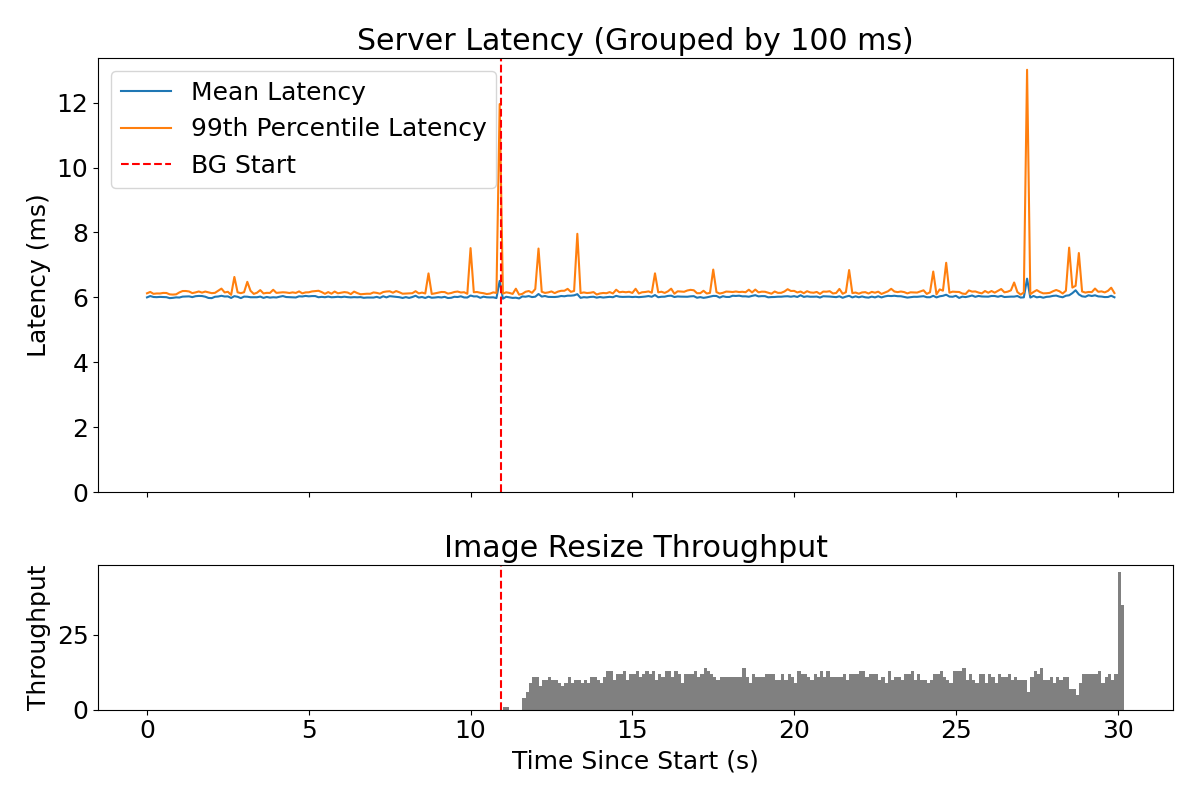
\includegraphics[width=\columnwidth]{graphs/srv-bg-schedbe-low.png}
        \caption{Low load}\label{fig:srv-bg-schedbe-low}
    \end{subfigure}
    \hspace{\fill}
    \begin{subfigure}[t]{0.49\columnwidth}
        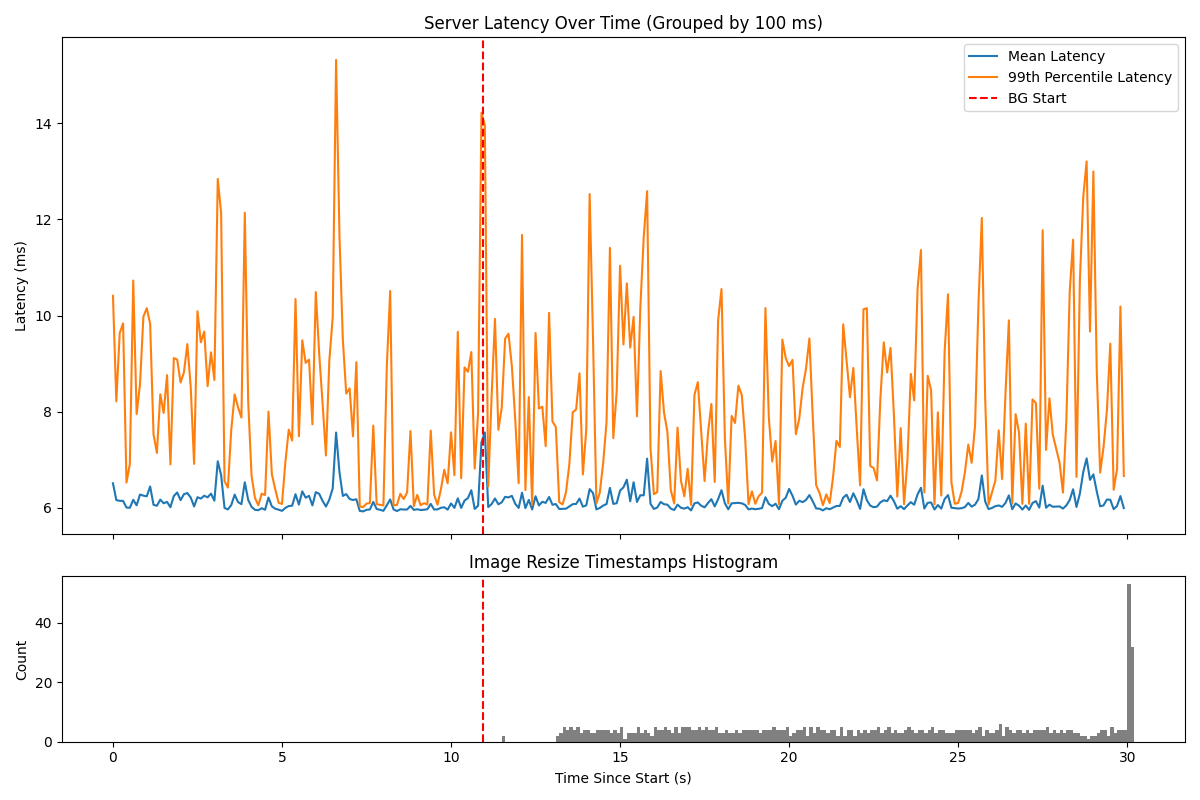
\includegraphics[width=\columnwidth]{graphs/srv-bg-schedbe-high.png}
        \caption{High load}\label{fig:srv-bg-schedbe-high}
    \end{subfigure}
    \vspace{4pt}
    \caption{same expiriment as in \autoref{fig:srv-bg-unedited}, but with the
    BEs running in \schedbe{}}\label{fig:srv-bg-schedbe}
\end{figure}

\begin{figure}[t]
    \centering
    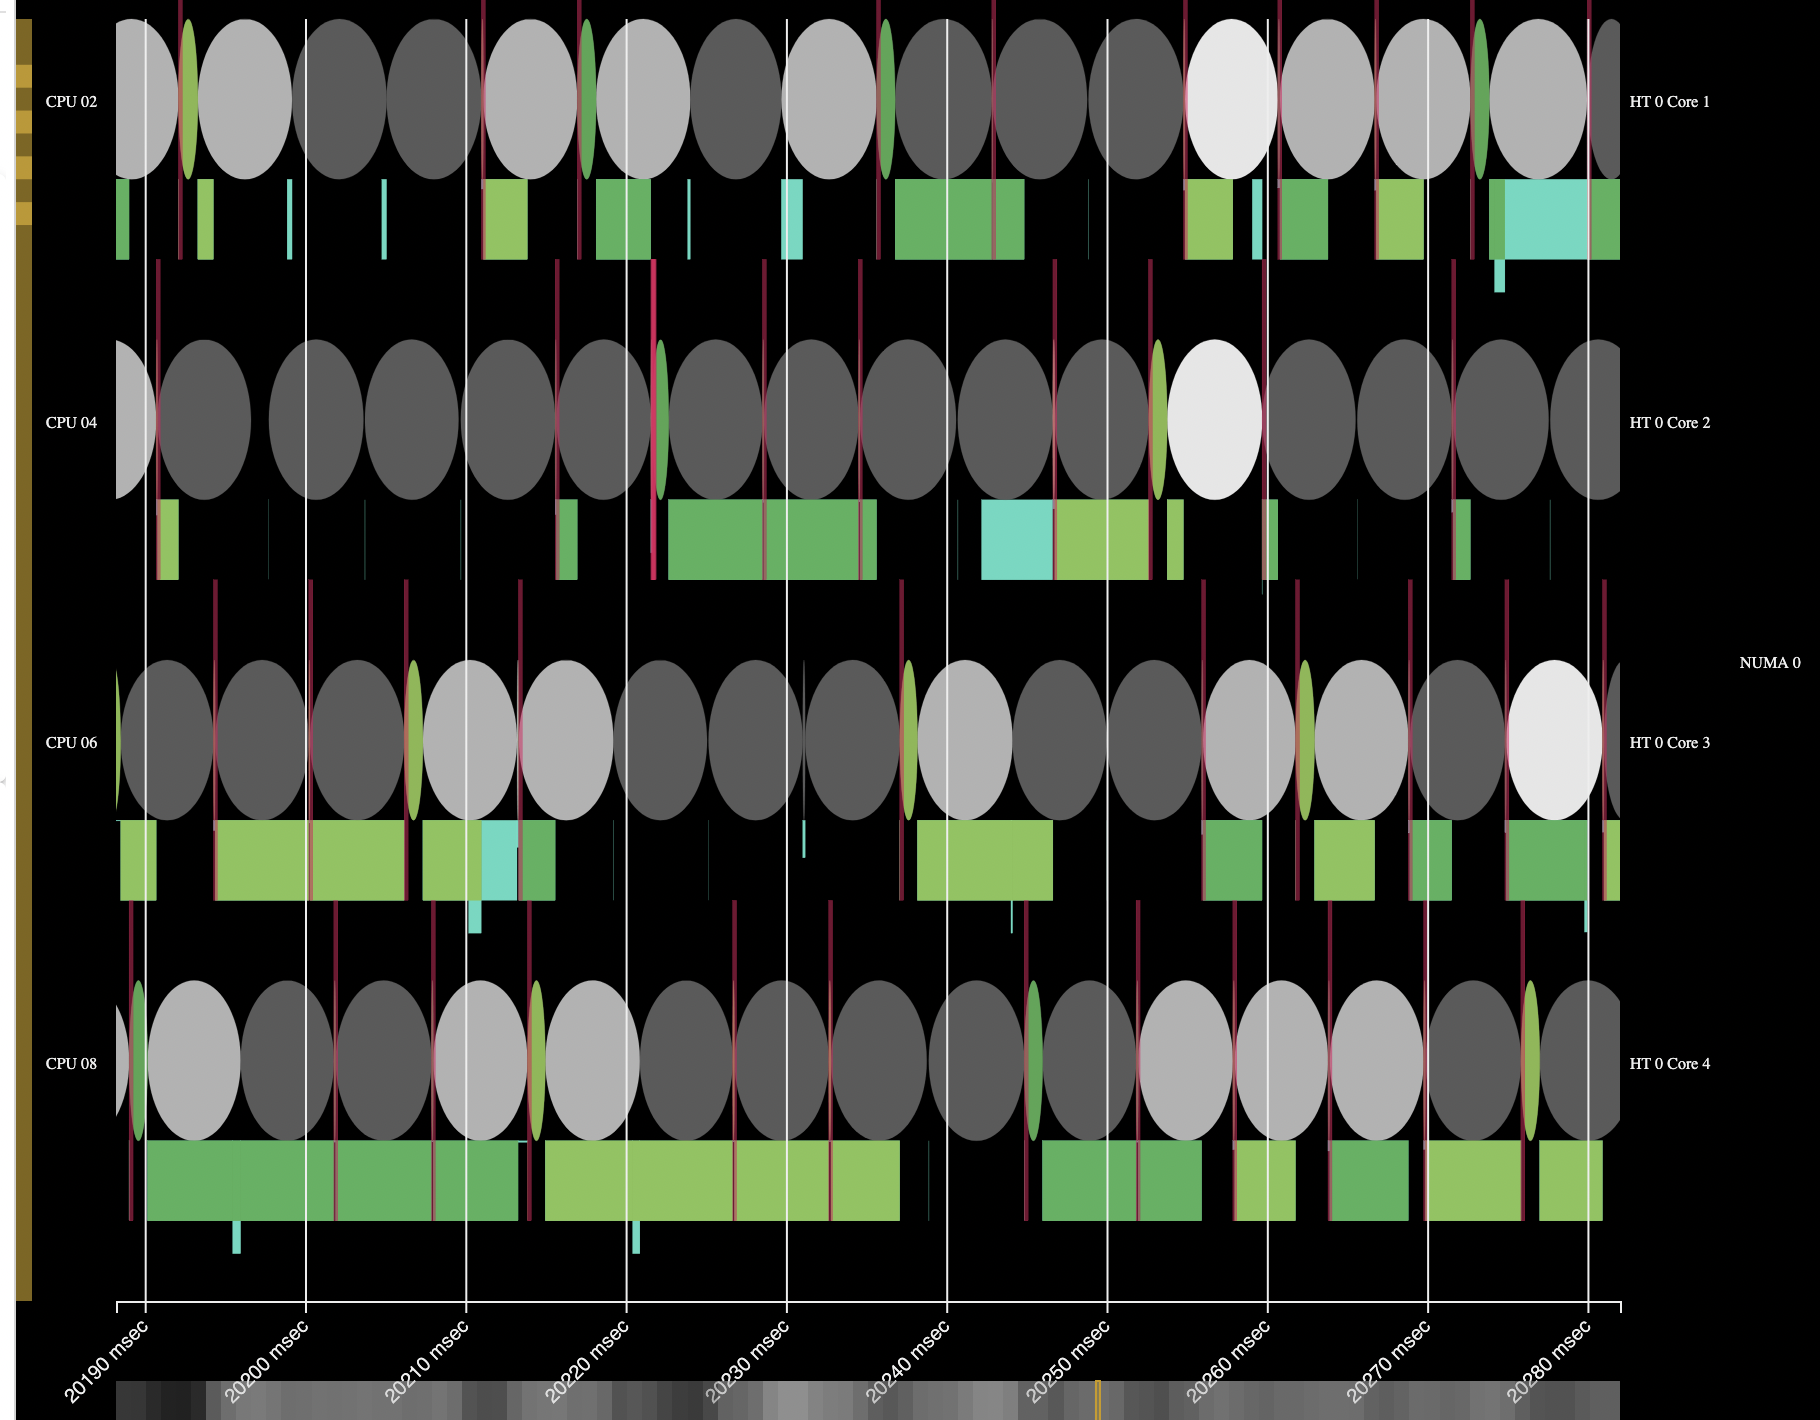
\includegraphics[width=\columnwidth]{graphs/schedviz-schedbe.png}
    \caption{The BE threads are colored in two different shades of green, the LC
    threads are the grey ones, the red vertical lines are the scheduler
    initially choosing a BE thread, which leads to an attempt to steal a queued
    LC one. As a result, BE threads only run when there are no queued LC
    threads.}\label{fig:schedviz-schedbe}
\end{figure}

We start by running the microbenchmark experiment using \schedbe{}. We use the
\cgroups{} interface to set the BE workloads to be marked as idle via the
\cgroups{} API, except that with the modified kernel that now puts the BE tasks
in \schedbe{}. We can see the resulting performance in
\autoref{fig:srv-bg-schedbe}. As desired the latency of the server remains
stable after the background tasks start. This does not mean that the background
task never runs: the lower graph still shows iterations of image resizing being
done. The difference is that now the background tasks will reliably get
interrupted when the LC server has a request to process. We can see this
happening in an outtake of the schedviz visualization in
\autoref{fig:schedviz-schedbe}. The green BE processes run only in the gaps
where there is no queued LC process, and are immediately preempted when one
wakes up, on whatever core that may be. The vertical red lines show when the
core has chosen intially to run a BE process. As we can see, this is sometimes
followed by just running the BE, but often by the core running an LC process,
meaning that it succesfully found and stole a queued and waiting LC thread.

\begin{figure}[t]
    \centering
    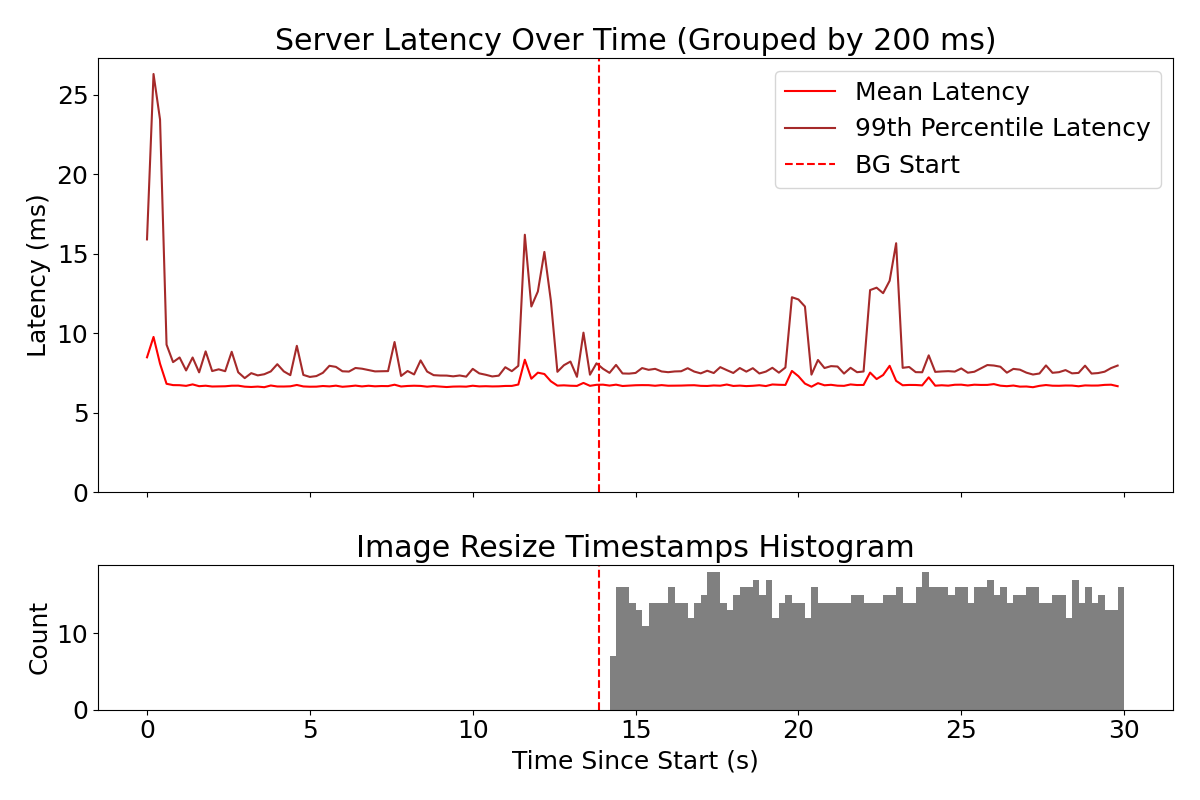
\includegraphics[width=\columnwidth]{graphs/kubernetes-schedbe.png}
    \caption{The same experiment as in \autoref{fig:kubernetes-unedited}, but
    running the BE as a \schedbe{} task}\label{fig:kubernetes-schedbe}
\end{figure}

We also run the Kubernetes application from \autoref{fig:kubernetes-unedited}
using \schedbe{}. We do this by explicitly setting the scheduling policy in the
BE code, rather than editing Kubernetes to change how it uses the \cgroups{}
API. The results are in \autoref{fig:kubernetes-schedbe}. We can see that, just
as in the microbenchmark, the latency profile of the web application looks
largely the same before and after starting the image resize job. It is not
entirely without spikes, but the spikes are the same before and after starting
the BE tasks and the baseline median latency stays stable. 

\subsection{Is parking necessary?}\label{ss:eval:parking}

Linux in its current form puts a high premium on ensuring every process in
guaranteed some amount of CPU time. As we saw earlier, real time applications
have strict priority in existing Linux and thus represent a possible antagonist
that would be able to starve everything else. However, Linux has two different
safeguards that protect against this. One is that \fifoclass{} is as a
scheduling class rate-limited: there are tuneable parameters at
\texttt{/proc/sys/kernel/sched\_rt\_runtime\_us} and
\texttt{/proc/sys/kernel/sched\_rt\_period\_us}, that together define a rate
limit for the \fifoclass{} class as a whole. The failsafes go further than just
that though: even when set to be equal (ie \fifoclass{} gets the full runtime
each period if it wants), the \normalclass{} scheduling class also has a
so-called \textit{deadline server}, which is basically a process is in the
\deadlineclass{} scheduling class with a small amount of runtime per
period~\cite{lkml-deadline-srv}. This deadline server is in essence a
representative of the \normalclass{} scheduling class, and when the
\deadlineclass{} scheduler runs the server, that hands control over to the
\normalclass{} scheduler, which picks a thread to run.


\begin{figure}[t]
    \centering
    \begin{subfigure}[t]{0.49\columnwidth}
        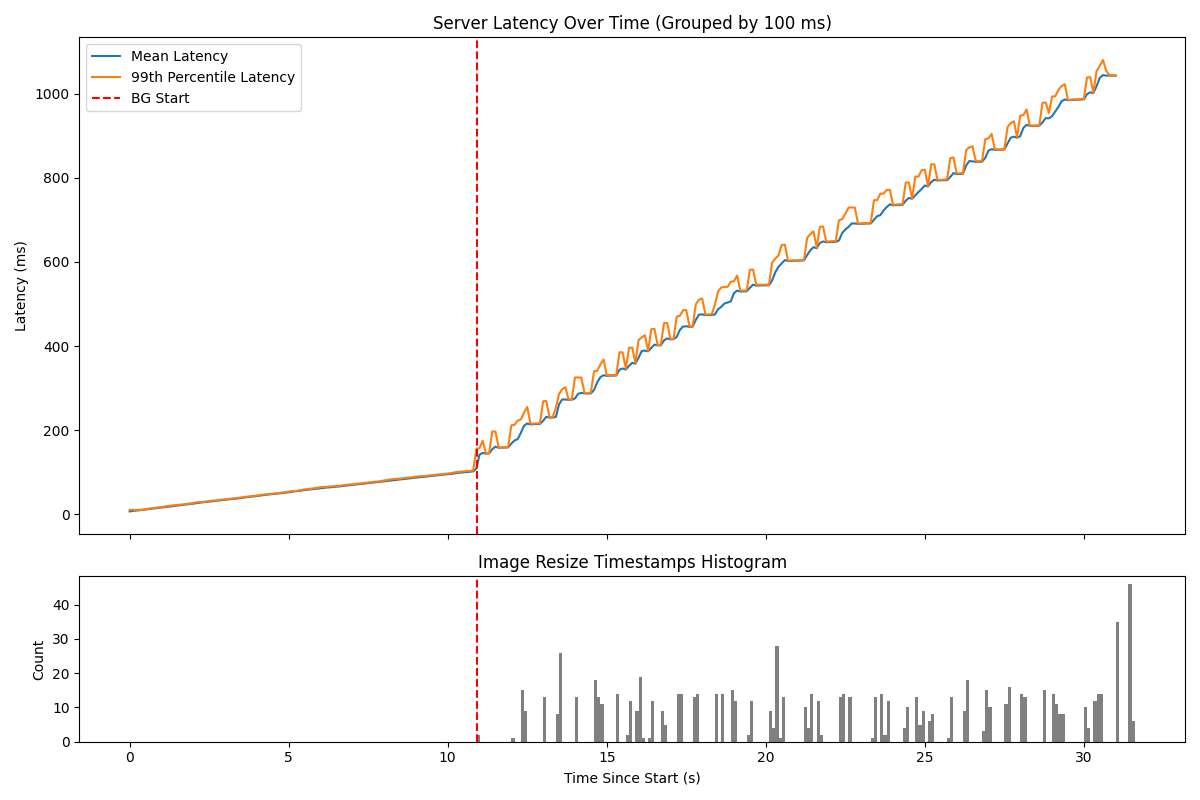
\includegraphics[width=\columnwidth]{graphs/overload-rt.png}
        \caption{LC in real time, throttling}\label{fig:overload-rt}
    \end{subfigure}
    \hspace{\fill}
    \begin{subfigure}[t]{0.49\columnwidth}
        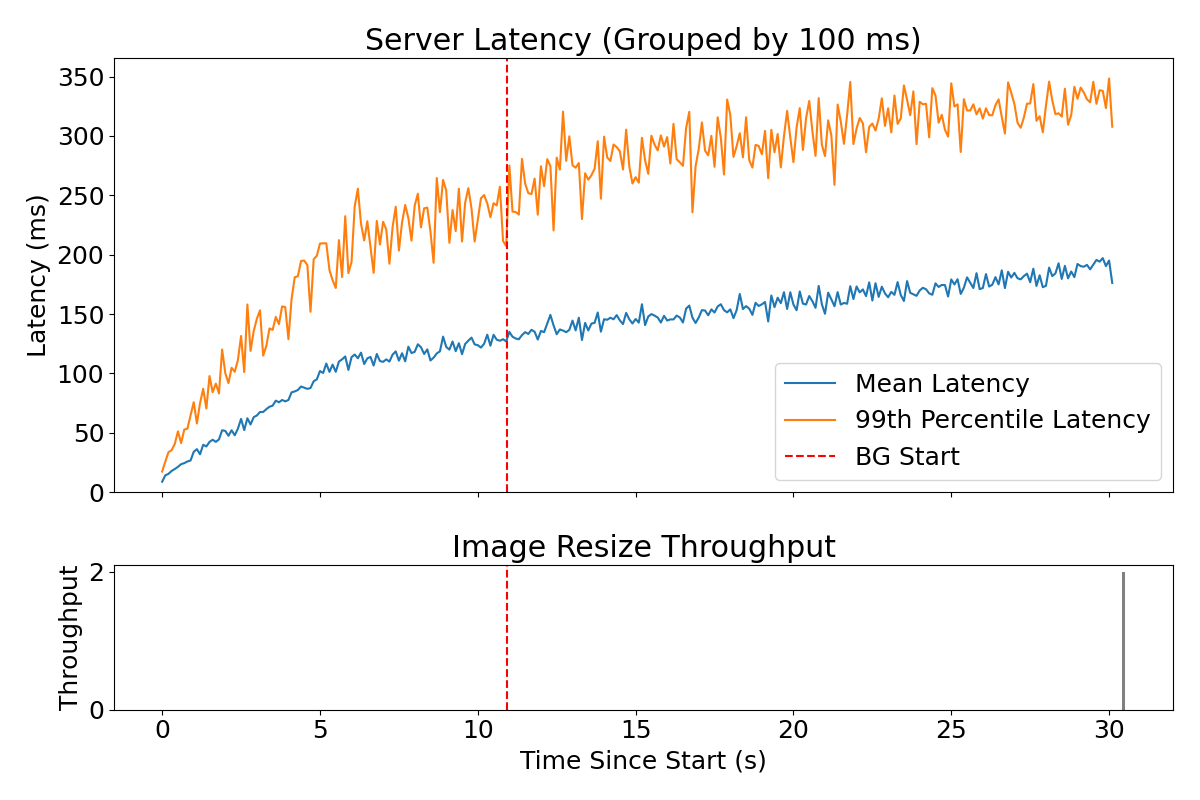
\includegraphics[width=\columnwidth]{graphs/overload-schedbe.png}
        \caption{BE in \schedbe{}, no throttling}\label{fig:overload-schedbe}
    \end{subfigure}
    \vspace{4pt}
    \caption{throttling the LC server under extremely high utilization, vs
    letting it starve the BE userspace processes}
\end{figure}


We can see this in action if we run the same microbenchmark experiment, but
instead of putting the LC server and BE resize jobs in different groups, we run
the LC in \fifoclass{} and the BE in \normalclass{}. To see the effects of the
throttling kicking in, we turn up the utilization: we run it so that the
baseline utilization is oversaturated (100\%). The results are in
\autoref{fig:overload-rt}. We see spikes begin to appear after starting the BE
task, because the \fifoclass{} server gets throttled in favor of running the BE
tasks; we see parallel spikes in the BE's throughpu in the bottom graph. Notice
also the increase of the slope of response times after starting the background
tasks: the deadline server mechanism only kicks in if there is load to run, so
once it does the resulting throttling degrades the servers performance
signigicantly. If this were taking place during a load spike while waiting for
new server instances to start, the presence of BE load would significantly
impact the queue length/performance degradation while the new server starts
up.\hmng{seems like a good experiment to do}

On the other hand, we see in \autoref{fig:overload-schedbe} what happens
if, in that same experiment, \schedbe{} allows the BE userspace process to be
parked. Notice that the BE does not make progress until the very end, when the
server is done processing the requests (the experiment stops the client after 30
seconds and the server from then finishes the backlog of requests).



\subsection{Cost of \schedbe{}}

We evaluate the cost of the additional checks required by \schedbe{} by looking
at how long the code takes to run, and how much lock contention it
creates.\hmng{This is a pretty big todo}




\subsection{Existing approaches}\label{ss:eval:existing}

To show the benefits of \schedbe{}, we compare with existing alternatives to
\cgroups{} within Linux.

\subsubsection{Realtime scheduling}

As we discussed in \autoref{s:solution}, Linux enforces the categorical
separation of tasks in different scheduling classes. 

This points to a possible alternative to using \cgroups{}: run LC in the
\fifoclass{} scheduling class and BE in \normalclass{}.\footnote{The
\deadlineclass{} scheduling class is not a good fit, since it requires accurate
knowledge of a processes runtime (processing time per request) and period (when
requests come in)} \fifoclass{} runs a priority scheduler: it has 99 priorities,
each takes strict precedent over the one lower; within priorities the scheduler
enforces a global first-in-first-out (hence the \fifoclass{} class name), based
on when processes become runnable.

\begin{figure}[t]
    \centering
    \begin{subfigure}[t]{0.48\columnwidth}
        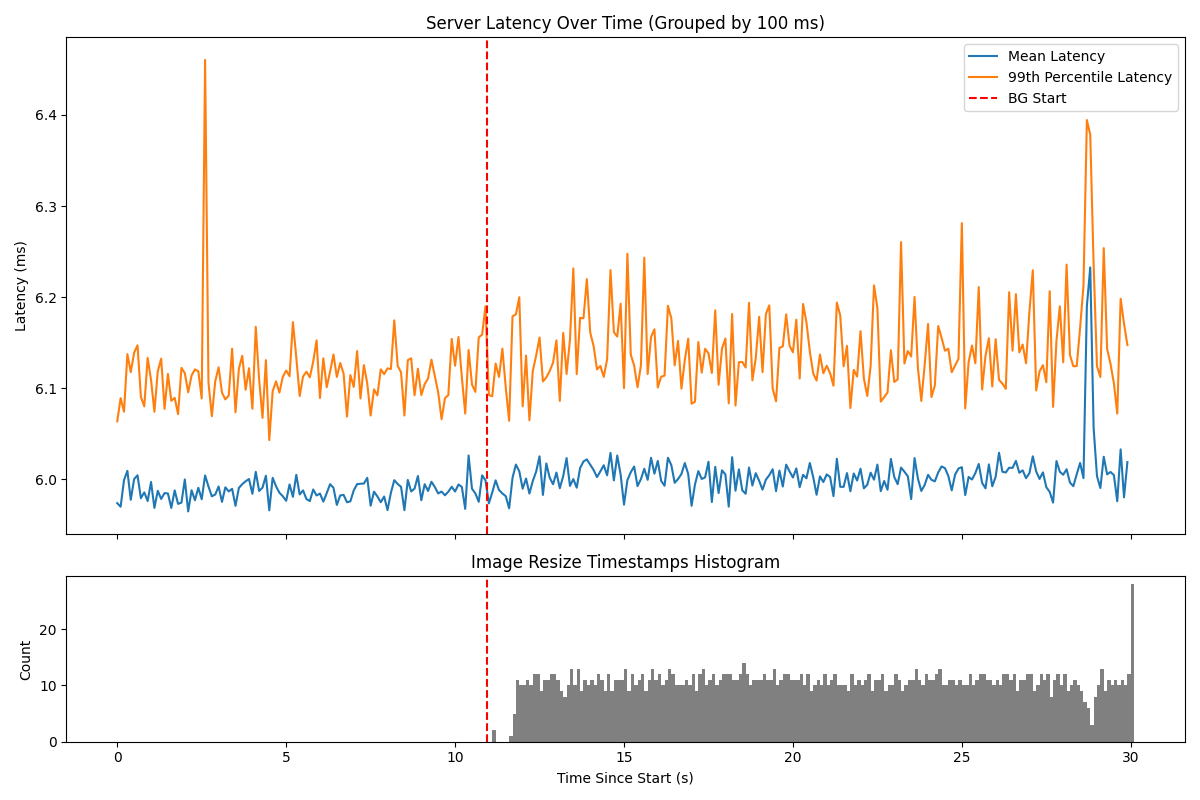
\includegraphics[width=\columnwidth]{graphs/srv-bg-rt-low.png}
        \caption{Low load}\label{fig:srv-bg-rt-low}
    \end{subfigure}
    \hspace{\fill}
    \begin{subfigure}[t]{0.48\columnwidth}
        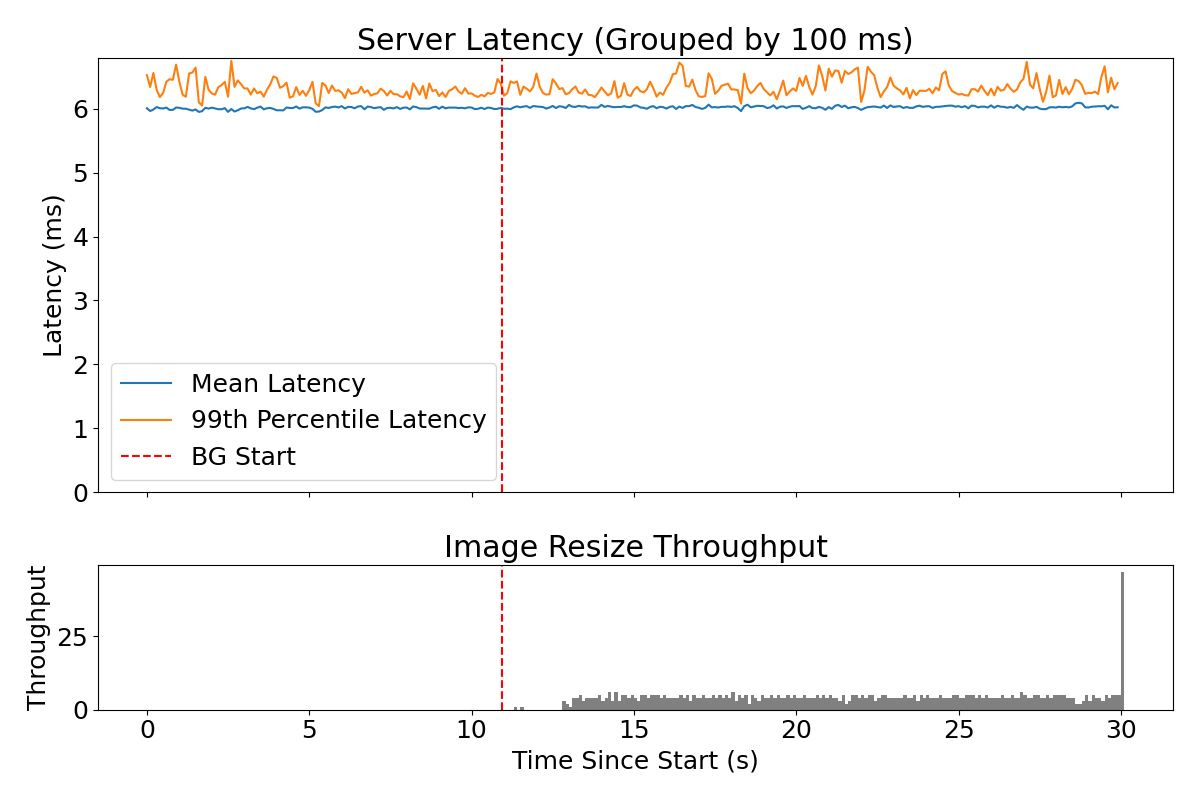
\includegraphics[width=\columnwidth]{graphs/srv-bg-rt-high.png}
        \caption{High load}\label{fig:srv-bg-rt-high}
    \end{subfigure}
    \vspace{4pt}
    \caption{Results of the same experiment as in \autoref{fig:srv-bg-unedited}
    and \autoref{fig:srv-bg-schedbe}, with LC running as a real time
    process}\label{fig:srv-bg-rt}
\end{figure}

We run the same microbenchmark experiment, but put the LC task in the
\fifoclass{} scheduling class, and leave BE tasks with the default
\normalclass{} scheduler and weight. \autoref{fig:srv-bg-rt} shows the resulting
measured latencies in the same low and high load setting as previously. As
expected, we see that Linux is able to isolate the two very well.

However, this is an untenable solution because of \fifoclass{}'s
run-to-completion scheduling, which is known to have a failure mode of
head-of-line (HoL) blocking under varied request processing times, where
long-running requests monopolize the CPU while short requests wait in the queue.
The \fifoclass{} scheduler also enforces not only cross-core isolation between
different priorities, but also a global ordering within the same priority. This
requires more synchronization, and is a stricter policy than we need.

The takeaway is that Linux's current mechanism of scheduling classes can isolate
workloads effectively, but existing scheduling classes use scheduling
algorithms that are not a good fit for modern workloads.

\subsubsection{\schedidle}\label{ss:schedidle}

As we discussed in \autoref{s:implementation}, \schedidle{} implements some but
not all of the isolation required of \beclass{}.

\begin{figure}[t]
    \centering
    \begin{subfigure}[t]{0.49\columnwidth}
        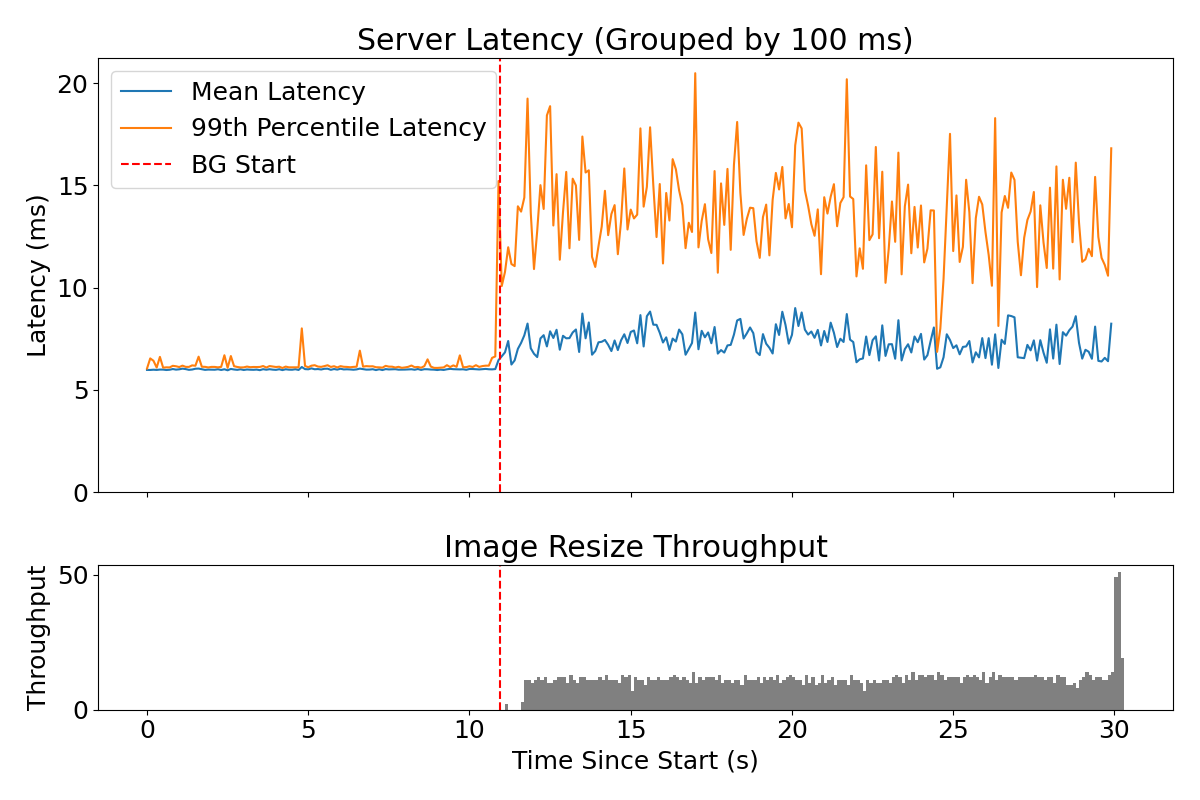
\includegraphics[width=\columnwidth]{graphs/srv-bg-idle-low.png}
        \caption{Low load}\label{fig:srv-bg-idle-low}
    \end{subfigure}
    \hspace{\fill}
    \begin{subfigure}[t]{0.49\columnwidth}
        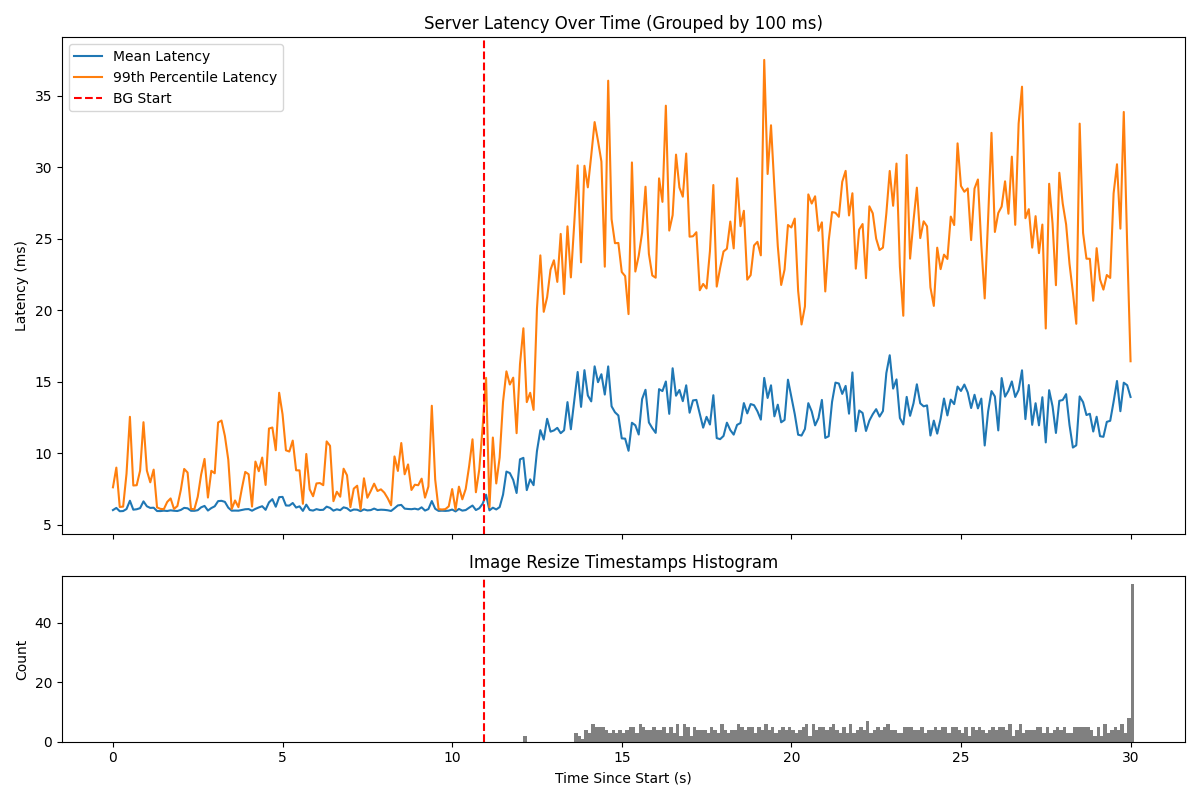
\includegraphics[width=\columnwidth]{graphs/srv-bg-idle-high.png}
        \caption{High load}\label{fig:srv-bg-idle-high}
    \end{subfigure}
    \vspace{4pt}
    \caption{using \schedidle{}}\label{fig:srv-bg-idle}
\end{figure}

And indeed, we find that when we use \cgroups{}' new cpu.idle interface feature,
the latency impact of the BE tasks decreases, although it does not entirely drop
to what we saw with the \fifoclass{} class, or with our \schedbe{} solution.\
\autoref{fig:srv-bg-idle} shows the results, for the familiar settings of low
and high load.